% Options for packages loaded elsewhere
\PassOptionsToPackage{unicode,linktoc=all}{hyperref}
\PassOptionsToPackage{hyphens}{url}
\PassOptionsToPackage{dvipsnames,svgnames,x11names}{xcolor}
%
\documentclass[
  a4paper,
]{article}
\usepackage{amsmath,amssymb}
\usepackage{lmodern}
\usepackage{iftex}
\ifPDFTeX
  \usepackage[T1]{fontenc}
  \usepackage[utf8]{inputenc}
  \usepackage{textcomp} % provide euro and other symbols
\else % if luatex or xetex
  \usepackage{unicode-math}
  \defaultfontfeatures{Scale=MatchLowercase}
  \defaultfontfeatures[\rmfamily]{Ligatures=TeX,Scale=1}
\fi
% Use upquote if available, for straight quotes in verbatim environments
\IfFileExists{upquote.sty}{\usepackage{upquote}}{}
\IfFileExists{microtype.sty}{% use microtype if available
  \usepackage[]{microtype}
  \UseMicrotypeSet[protrusion]{basicmath} % disable protrusion for tt fonts
}{}
\makeatletter
\@ifundefined{KOMAClassName}{% if non-KOMA class
  \IfFileExists{parskip.sty}{%
    \usepackage{parskip}
  }{% else
    \setlength{\parindent}{0pt}
    \setlength{\parskip}{6pt plus 2pt minus 1pt}}
}{% if KOMA class
  \KOMAoptions{parskip=half}}
\makeatother
\usepackage{xcolor}
\IfFileExists{xurl.sty}{\usepackage{xurl}}{} % add URL line breaks if available
\IfFileExists{bookmark.sty}{\usepackage{bookmark}}{\usepackage{hyperref}}
\hypersetup{
  pdftitle={What Ails Indian Education?},
  pdfauthor={R (Chandra) Chandrasekhar},
  pdflang={en-GB},
  colorlinks=true,
  linkcolor={DarkOliveGreen},
  filecolor={Purple},
  citecolor={DarkKhaki},
  urlcolor={Maroon},
  pdfcreator={LaTeX via pandoc}}
\urlstyle{same} % disable monospaced font for URLs
\usepackage[margin=25mm]{geometry}
\usepackage{graphicx}
\makeatletter
\def\maxwidth{\ifdim\Gin@nat@width>\linewidth\linewidth\else\Gin@nat@width\fi}
\def\maxheight{\ifdim\Gin@nat@height>\textheight\textheight\else\Gin@nat@height\fi}
\makeatother
% Scale images if necessary, so that they will not overflow the page
% margins by default, and it is still possible to overwrite the defaults
% using explicit options in \includegraphics[width, height, ...]{}
\setkeys{Gin}{width=\maxwidth,height=\maxheight,keepaspectratio}
% Set default figure placement to htbp
\makeatletter
\def\fps@figure{htbp}
\makeatother
\setlength{\emergencystretch}{3em} % prevent overfull lines
\providecommand{\tightlist}{%
  \setlength{\itemsep}{0pt}\setlength{\parskip}{0pt}}
\setcounter{secnumdepth}{-\maxdimen} % remove section numbering
\newlength{\cslhangindent}
\setlength{\cslhangindent}{1.5em}
\newlength{\csllabelwidth}
\setlength{\csllabelwidth}{3em}
\newlength{\cslentryspacingunit} % times entry-spacing
\setlength{\cslentryspacingunit}{\parskip}
\newenvironment{CSLReferences}[2] % #1 hanging-ident, #2 entry spacing
 {% don't indent paragraphs
  \setlength{\parindent}{0pt}
  % turn on hanging indent if param 1 is 1
  \ifodd #1
  \let\oldpar\par
  \def\par{\hangindent=\cslhangindent\oldpar}
  \fi
  % set entry spacing
  \setlength{\parskip}{#2\cslentryspacingunit}
 }%
 {}
\usepackage{calc}
\newcommand{\CSLBlock}[1]{#1\hfill\break}
\newcommand{\CSLLeftMargin}[1]{\parbox[t]{\csllabelwidth}{#1}}
\newcommand{\CSLRightInline}[1]{\parbox[t]{\linewidth - \csllabelwidth}{#1}\break}
\newcommand{\CSLIndent}[1]{\hspace{\cslhangindent}#1}
\ifLuaTeX
\usepackage[bidi=basic]{babel}
\else
\usepackage[bidi=default]{babel}
\fi
\babelprovide[main,import]{british}
% get rid of language-specific shorthands (see #6817):
\let\LanguageShortHands\languageshorthands
\def\languageshorthands#1{}
% $HOME/.pandoc/defaults/latex-header-includes.tex
% Common header includes for both lualatex and xelatex engines.
%
% Preliminaries
%
\PassOptionsToPackage{rgb,dvipsnames,svgnames}{xcolor}
\PassOptionsToPackage{main=british}{babel}
\AtBeginEnvironment{quote}{\small}
\AtBeginEnvironment{quotation}{\small}
\AtBeginEnvironment{longtable}{\centering}
%
% Packages that are useful to include
%
\usepackage{graphicx}
\usepackage{subcaption}
\usepackage[inkscapeversion=1]{svg}
\usepackage[defaultlines=4,all]{nowidow}
\usepackage[capitalize,noabbrev]{cleveref}
\usepackage{etoolbox}
\usepackage{fontsize}
\usepackage{newunicodechar}
\usepackage{pdflscape}
\usepackage{fnpct}
\usepackage{parskip}
  \setlength{\parindent}{0pt}
\usepackage[style=american]{csquotes}

% charis-plus.tex
% Font-setting header file for use with Pandoc Markdown
% to generate PDF via LuaLaTeX.
% The main font is Charis SIL.
% Other main fonts are also available in appropriately named file.
\usepackage{fontspec}
\usepackage{setspace}
\setstretch{1.2}
%
\defaultfontfeatures{Ligatures=TeX,Scale=MatchLowercase} % at the start always
%
% For English
%
\babelfont{rm}[Scale=1]{Merriweather}
\babelfont{sf}[BoldFont={* Semibold}]{Source Sans Pro}
\babelfont{tt}[Scale=0.9]{Fira Mono}
%
\babelprovide[import,onchar=ids fonts]{sanskrit}
\babelprovide[import,onchar=ids fonts]{tamil}
\babelprovide[import,onchar=ids fonts]{greek}
%
\babelfont[sanskrit]{rm}[Scale=1.1,Renderer=HarfBuzz]{Noto Serif Devanagari}
\babelfont[sanskrit]{sf}[Scale=1.1,Renderer=HarfBuzz]{Noto Sans Devanagari}
\babelfont[tamil]{rm}[Renderer=HarfBuzz]{Noto Serif Tamil}
\babelfont[tamil]{sf}[Renderer=HarfBuzz]{Noto Sans Tamil}
\babelfont[greek]{rm}{Gentium Book Plus}
%
% Math font
%
\usepackage{unicode-math} % seems not to hurt % fallabck
\setmathfont[bold-style=TeX]{STIX Two Math}
%
% Other fonts
%
\newfontfamily{\emojifont}{Symbola}
%
\usepackage{titling}
\usepackage{fancyhdr}
    \pagestyle{fancy}
    \fancyhead{}
    \fancyfoot{}
    \renewcommand{\headrulewidth}{0.2pt}
    \renewcommand{\footrulewidth}{0.2pt}
    \fancyhead[LO,RE]{\scshape\thetitle}
    \fancyfoot[CO,CE]{\footnotesize Copyright © 2006\textendash\the\year, R (Chandra) Chandrasekhar}
    \fancyfoot[RE,RO]{\thepage}
\newfontfamily{\regulariconfont}{Font Awesome 6 Free Regular}[Color=Grey]
\newfontfamily{\solidiconfont}{Font Awesome 6 Free Solid}[Color=Grey]
\newfontfamily{\brandsiconfont}{Font Awesome 6 Brands}[Color=Grey]
%
% Direct input of Unicode code points
%
\newcommand{\faEnvelope}{\regulariconfont\ ^^^^f0e0\normalfont}
\newcommand{\faMobile}{\solidiconfont\ ^^^^f3cd\normalfont}
\newcommand{\faLinkedin}{\brandsiconfont\ ^^^^f0e1\normalfont}
\newcommand{\faGithub}{\brandsiconfont\ ^^^^f09b\normalfont}
\newcommand{\faAtom}{\solidiconfont\ ^^^^f5d2\normalfont}
\newcommand{\faPaperPlaneRegular}{\regulariconfont\ ^^^^f1d8\normalfont}
\newcommand{\faPaperPlaneSolid}{\solidiconfont\ ^^^^f1d8\normalfont}

%
% The block below is commented out because of Tofu glyphs in HTML
%
% \newcommand{\faEnvelope}{\regulariconfont\ \normalfont}
% \newcommand{\faMobile}{\solidiconfont\ \normalfont}
% \newcommand{\faLinkedin}{\brandsiconfont\ \normalfont}
% \newcommand{\faGithub}{\brandsiconfont\ \normalfont}
\ifLuaTeX
  \usepackage{selnolig}  % disable illegal ligatures
\fi

\title{What Ails Indian Education?}
\author{R (Chandra) Chandrasekhar}
\date{2013-09-18 | 2022-05-26}

\begin{document}
\maketitle




\begin{quote}
This blog was originally written in 2013 when the links giving the
rankings were active. They have now faded away into cyber-oblivion, but
might be restored in future. It bears noting that some Indian
universities have improved their global rankings since.
\end{quote}

\hypertarget{no-place-at-the-top}{%
\subsection{No place at the top}\label{no-place-at-the-top}}

The
\href{http://www.topuniversities.com/university-rankings/world-university-rankings/2013\#sorting=rank+region=+country=+faculty=+stars=false+search=}{QS
World University rankings for 2013} have just been released. This is one
of several league tables ranking universities according to various
criteria of academic performance. Such rankings are symptomatic of the
relentless trend to quantify more and more aspects of our lives. May
this madness be checked before intangible attributes best left
qualitative---like love and loyalty---are also subjected to mindless,
simplistic metrology!

These world rankings have generated a collective
\href{http://articles.timesofindia.indiatimes.com/2013-09-11/news/41969629_1_qs-world-university-rankings-mumbai-university-indian}{disquiet}
that not a single university in India is featured in the top 200
universities worldwide.

This topical fact set me thinking about what ails the Indian education
system in general. While I cannot lay claim to hard facts backing my
opinions, personal anecdotal evidence points to a steep and startling
decline in Indian educational standards in the opening decades of the
twenty-first century. The Indian graduates of yesteryear were made of
sterner stuff, intellectually speaking.

\hypertarget{money-as-the-highest-good}{%
\subsection{Money as the highest good}\label{money-as-the-highest-good}}

One factor contributing to the decline is the obvious present day
malaise afflicting Indian society at large, where money has become the
highest good, period. That unthinking, unregenerate, single-minded
fixation on money has kicked out the \emph{l} in \emph{learning} to
yield \emph{earning} as the primary goal of the Indian student---whether
in school or at college.

Notwithstanding this tragic, amoral mindset, and quite distinct from the
economic, political, and social morass waiting to gobble up the young
high school or university graduate, there is, I think a deeper ailment
plaguing education in India today. Predictably, it is rooted in India's
past. And paradoxically, it springs from the Vedic tradition, where the
Sanskrit word \emph{Veda} literally means \emph{knowledge.}

\hypertarget{the-preservation-of-vedic-knowledge}{%
\subsection{The preservation of Vedic
knowledge}\label{the-preservation-of-vedic-knowledge}}

The \href{http://en.wikipedia.org/wiki/Vedas}{Vedas} originated in a
period before a written script was available to accommodate that
knowledge, phrased in the precursor to the classical
\href{http://en.wikipedia.org/wiki/Sanskrit}{Sanskrit} studied today.
The Vedas were set to metre to aid in singing or reciting them, and
ingenious means were devised to ensure textual correctness, including
probably the most scientific rules of euphony, or
\href{https://en.wikipedia.org/wiki/Sandhi}{\emph{sandhi}}, ever devised
for a natural language.

Lacking a script that could store the Vedic lore, the ancients decided
to use the human brain and its temporally intransigent abstraction---the
human mind---as distributed storage media. The Vedas were literally
preserved as memories in human minds and bequeathed from one generation
of scholar-priests to the next.

This is not a unique achievement---witness the Norse sagas and the
ancient mythology of most cultures which have also been orally
transmitted down the ages. But the Vedas enjoy an additional, singular
distinction: they have been preserved almost error-free from the hoary
times when they were first recited, by virtue of the almost mathematical
rigour that Sanskrit embodies for its grammar and phonetics, not to
mention mnemonics \protect\hyperlink{ref-bhatekak1993}{{[}1{]}}.

\begin{figure}
\hypertarget{fig:teacher-students}{%
\centering
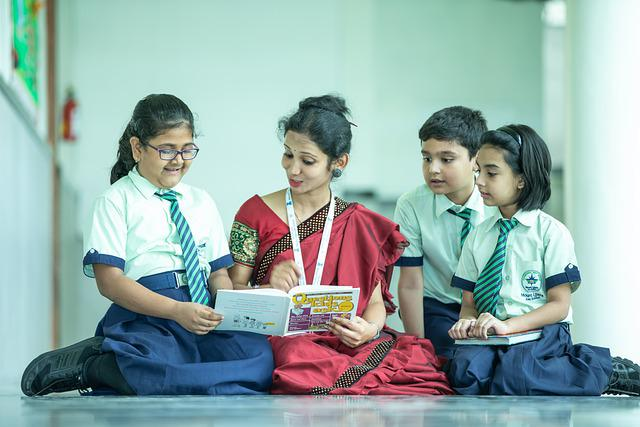
\includegraphics[width=0.8\textwidth,height=\textheight]{images/school-ga9b21f7d6_640.jpg}
\caption[Teacher with students in India.]{Teacher with students in
India.\footnotemark{}}\label{fig:teacher-students}
}
\end{figure}
\footnotetext{Image by
  \href{https://pixabay.com/users/anilsharma26-13475484/}{Anil Sharma}
  from \href{https://pixabay.com/}{Pixabay}.}

\hypertarget{memorization-as-the-great-bane}{%
\subsection{Memorization as the great
bane}\label{memorization-as-the-great-bane}}

The upshot of this ``mind over matter'' preservation of the Vedas was
that \emph{memorization and scholarship became fused in Indian culture.}
This is a fundamental drawback that trips the contemporary Indian
student. Rather than developing the ability to think logically and
independently, she or he is encouraged by parents, teachers, and the
system in general, to memorize knowledge and parrot it out in an
examination: something which is charmingly described as the \emph{commit
and vomit} method.

One is reminded here of these lines from Tennyson's \emph{Morte
D'Arthur}:

\begin{quote}
The old order changeth, yielding place to new,\\
And God fulfils Himself in many ways,\\
Lest one good custom should corrupt the world.
\end{quote}

Mark that I am not against developing a good memory or exercising it to
keep fit mentally. Indeed, in my chapters entitled ``Poetry'' and
``Arithmetic Revisited''---from the manuscript of my forthcoming book
\href{\%7Bstatic\%7D/sas-manuscript/SAS-partial.pdf}{\emph{Secrets of
Academic Success}}---I have suggested poetry recitation and mental
arithmetic as ways to develop memory while at the same time becoming
more literate and numerate.

In any case, developing a good memory is quite distinct from memorizing
facts without understanding them. The legendary Albert Einstein is
reputed to have advised,
\href{http://en.wikiquote.org/wiki/Albert_Einstein}{``Never memorize
what you can look up in books.''} His words ring even more true today,
when so much information is available from the Web, literally at the
click of a mouse button.

Memorization can scarce supplant the ability to think independently, or
critically, or afresh. Alas, in India, recall has replaced
understanding. A dozen years of education produce trained parrots rather
than thinking human beings capable of dealing with the unforeseen and
unforeseeable challenges of the future.

Despite the
\href{http://deedy.quora.com/Hacking-into-the-Indian-Education-System}{rot}
that is periodically revealed about examinations in India, they enjoy
sacred status in the minds of parents and, by transitivity, students.
Rank---that fateful word again for position in a sequence---means
everything. To top an examination---by memorization rather than
thinking---thus becomes the Holy Grail of an earnest student nurtured on
the soil of academe in India. This, I consider the first great bane in
the Indian education system.

\hypertarget{the-teacher-as-a-god}{%
\subsection{The teacher as a god}\label{the-teacher-as-a-god}}

The Vedic tradition is responsible for another practice that has
unfortunately been extrapolated without wisdom. The teacher was accorded
a veneration second to none in society, and a status akin to a god. What
was not grasped in all its subtlety was that this respect was given to
an \emph{enlightened teacher,} and if that phrase causes you to wrinkle
your brows in confusion, think of the Buddha, as a historically proximal
example. \emph{He} merited veneration. But the unthinking pursuit of
this tradition has meant that \emph{all} teachers---spiritual and
secular, enlightened and deluded---are accorded a god-like status,
irrespective of their knowledge, merits, or worth.

In this context, I remember an anecdote recounted by a friend of mine.
When the economist
\href{http://en.wikipedia.org/wiki/John_Kenneth_Galbraith}{John Kenneth
Galbraith} arrived in India as President Kennedy's ambassador to India,
he was pleasantly shocked when the receiving Indian official prostrated
himself fully on the floor before the astonished professor, telling him
that, as he had learned economics from Galbraith's textbooks, he was
giving him the respect due to a teacher or \emph{guru} in India.
Apocryphal or not, and without prejudice to Galbraith's personal merit,
this story well illustrates the \emph{automatic} adulation accorded a
teacher in India.

\hypertarget{debate-and-knowledge}{%
\subsection{Debate and knowledge}\label{debate-and-knowledge}}

The tradition of democracy developed in the West embraces adversarial
debate as its basis in parliament. In similar fashion, the scientific
paradigm in place today requires the practitioner to challenge the
status quo. The reason is simple: there is no finality in science or
medicine. These are disciplines where there is no conclusive,
indisputable truth as in mathematics. There are only ever closer
approximations to reality.

Thus it was that Einstein unseated Newton as the reigning monarch of
time, space, and gravity after three hundred years. And surely, there
will be another who will dethrone Einstein in time to come.

Let me digress now to give you another anecdote. While on my evening
constitutional one day, I fell in step with an Indian student completing
a postgraduate degree in the life sciences. He was intelligent and
articulate, and preparing some papers for publication that would be his
passport to a PhD programme at an overseas university.

I inquired generally about his work and the research climate in his
department and laboratory. He suddenly became animated and told me
dolefully, ``If the professor says that dogs have three legs, we must
nod in pliant agreement, not dispute and debate to establish the
truth.'' Whether this statement originated from the ``teacher is a god''
tradition of India, or was a sarcastic barb on professorial omniscience
in Indian academia, I know not. But the Indian student, whether stymied
by reverence for the godly instructor, or subdued into silence by
prudent self-survival, is ill-suited to questioning the received wisdom
in contemporary science and medicine.

This environment which inhibits a student from questioning or
challenging the status quo is the second great failing in the Indian
education system. And paradoxically, it is antithetical to the Vedic
tradition whose great
\href{http://en.wikipedia.org/wiki/Upanishads}{Upanishads} were
treatises born of enquiry, bold and uncircumscribed. How strange that
both problem and solution stem from the same scriptures!

\hypertarget{fun-imagination-and-learning}{%
\subsection{Fun, imagination, and
learning}\label{fun-imagination-and-learning}}

To free the Indian education system from its constraining shackles,
learning must become fun once more. Pedagogy must be reformed to allow
this. Each and every child is imbued with a natural and insatiable
curiosity. If only early childhood education could be ameliorated to
fuel rather than extinguish this spark, Mother Nature will do the rest.

Rote memorization cannot and should not be equated with learning and
knowledge. Examinations and other methods of assessment should be
designed with this goal in mind. They should test understanding in
preference to recall.

Imagination must be fostered because it is the fount of all new
knowledge. Who could have \emph{imagined} that Nature would exhibit
\href{http://www.youtube.com/watch?v=0Eeuqh9QfNI\&list=TLlNpED2t9U9sv5MXb2p3Bdqhg2XFcWnBG}{quantum
entanglement} or that the brain is
\href{http://faculty.washington.edu/chudler/plast.html}{neuroplastic} or
that carbon, already known to us as diamond and graphite, would disguise
itself yet again to appear as
\href{http://en.wikipedia.org/wiki/Bucky_balls}{Buckyballs} and
\href{http://www.graphene.manchester.ac.uk/}{graphene}? Knowledge
confines us to discovered facts. Imagination liberates us to find new
ones.

The thrill of discovery and the unleashing of the imagination---to
discover lands undreamed of---must fuel the education, not just of the
Indian student, but of all humankind. Education \emph{must} be reformed
to accomplish this.

\hypertarget{feedback}{%
\subsection{Feedback}\label{feedback}}

Please \href{mailto:feedback.swanlotus@gmail.com}{email me} your
comments and corrections.

\noindent A PDF version of this article is
\href{./what-ails-indian-education.pdf}{available for download here:}

\begin{normalsize}

\begin{ttfamily}

\url{https://swanlotus.netlify.app/blogs/what-ails-indian-education.pdf}

\end{ttfamily}

\end{normalsize}

\hypertarget{bibliography}{%
\section*{References}\label{bibliography}}
\addcontentsline{toc}{section}{References}

\hypertarget{refs}{}
\begin{CSLReferences}{0}{0}
\leavevmode\vadjust pre{\hypertarget{ref-bhatekak1993}{}}%
\CSLLeftMargin{{[}1{]} }
\CSLRightInline{S. Bhate and S. Kak, {`{Pāṇini's Grammar and Computer
Science}'}, \emph{Annals of the Bhandarkar Oriental Research Institute},
vol. 72, pp. 79--94, 1993. }

\end{CSLReferences}



\end{document}
